\chapter{Resultados e Discussão}

Este capítulo detalha os experimentos realizados e analisa a eficácia da arquitetura proposta. Diferente de ambientes controlados com \textit{datasets} maduros, os resultados aqui apresentados refletem os desafios reais de uma rede social em fase de crescimento (Bluesky), onde a escassez de interações topológicas impacta diretamente a precisão dos modelos de grafos.

\section{O Problema da Transferência de Domínio (Twitter vs. Bluesky)}

O primeiro grande experimento consistiu no ``Duelo de Modelos'', testando a capacidade de generalização. Utilizou-se o modelo treinado com o \textit{benchmark} UPFD (originário do Twitter) para classificar dados nativos do Bluesky.

\begin{figure}[htb]
    \centering
    \caption{Matriz de Confusão: Modelo UPFD aplicado ao Bluesky Aberto}
    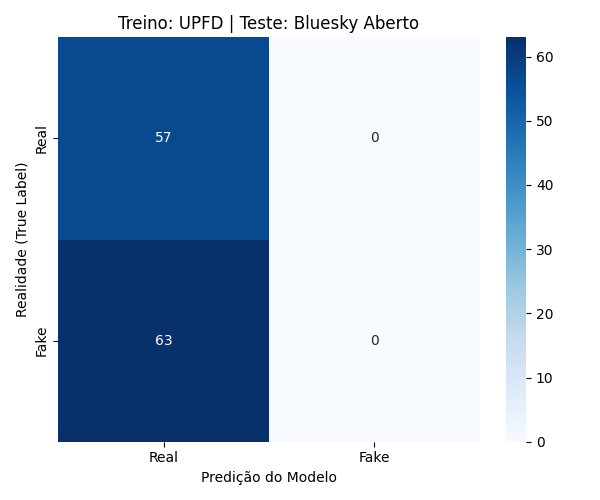
\includegraphics[width=0.7\textwidth]{Imagens/matriz_upfd_vs_bs_aberto.png}
    \fonte{Elaborado pelos autores (2026).}
\end{figure}

Conforme evidenciado na Figura acima, o desempenho foi insatisfatório. O modelo tendeu a classificar a grande maioria das postagens como ``Real'', resultando em uma taxa nula de detecção de \textit{fake news} no ambiente aberto. Esse fenômeno valida a hipótese de que a desinformação é contextual: as métricas de velocidade e profundidade que definem uma notícia falsa no Twitter não se traduzem diretamente para o Bluesky, devido à diferença na densidade da rede e no comportamento dos usuários.

\section{Desempenho Nativo e o Desafio do ``Cold Start''}

Ao treinar e testar o modelo exclusivamente com dados do Bluesky, observou-se uma melhora, porém com limitações.

\begin{figure}[htb]
    \centering
    \caption{Matriz de Confusão: Treino e Teste Nativo no Bluesky (Controlado)}
    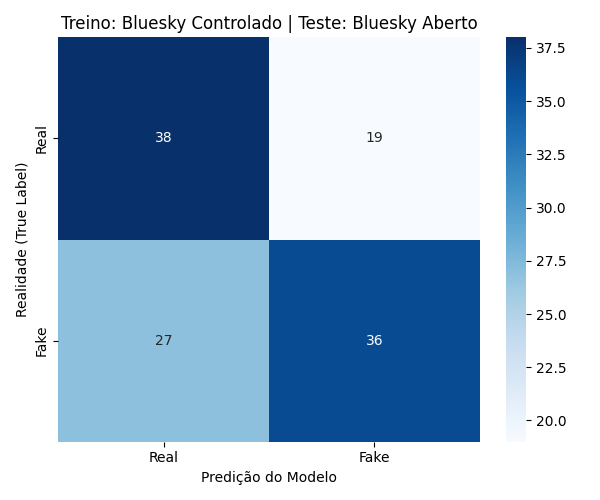
\includegraphics[width=0.7\textwidth]{Imagens/matriz_bs_ctrl_vs_bs_aberto.png}
    \fonte{Elaborado pelos autores (2026).}
\end{figure}

A análise da Matriz de Confusão revela um equilíbrio tênue, com uma quantidade considerável de falsos positivos (27) e falsos negativos (19). Este resultado intermediário é atribuído à natureza da rede analisada. Por ser uma plataforma descentralizada e relativamente nova, o Bluesky apresenta o ``abismo de generalização''. A falta de uma estrutura de grafos densa impede que a GCN explore plenamente a geometria da disseminação.

\section{Impacto do Ceticismo: Ajuste de Penalidade}

Para superar as limitações do modelo controlado, testou-se a estratégia de penalização progressiva de falsos positivos durante o treinamento. A hipótese era que um modelo treinado para ser mais ``cético'' --- ou seja, punindo mais severamente a classificação incorreta de \textit{fake news} como real --- apresentaria melhor desempenho no ambiente aberto do Bluesky.

\begin{figure}[htb]
    \centering
    \caption{Matriz de Confusão: Modelo Exageradamente Cético aplicado ao Bluesky Aberto}
    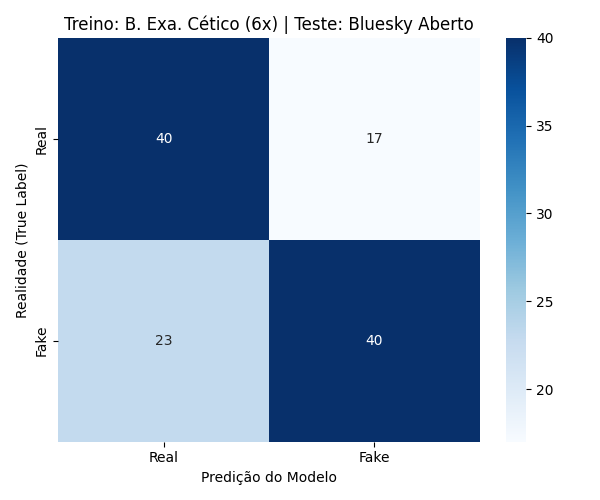
\includegraphics[width=0.7\textwidth]{Imagens/matriz_bs_exa_cetico_vs_bs_aberto.png}
    \fonte{Elaborado pelos autores (2026).}
\end{figure}

Os resultados confirmam a hipótese: o modelo Exageradamente Cético, treinado com penalidade sêxtupla (6x) para falsos negativos, apresentou a menor taxa de \textit{fake news} não detectadas. Este modelo recebe, consequentemente, o maior peso (40\%) no \textit{ensemble} final.

\section{O Framework de Ensemble Ponderado}

A síntese dos experimentos anteriores resultou na proposta central deste trabalho: ao invés de confiar em um único modelo, o sistema combina os quatro classificadores em um \textit{framework} de votação ponderada. Os pesos foram definidos com base no desempenho empírico de cada modelo:

\begin{table}[htb]
    \centering
    \caption{Composição do Framework de Ensemble}
    \begin{tabular}{|l|c|l|}
        \hline
        \textbf{Modelo} & \textbf{Peso} & \textbf{Justificativa} \\
        \hline
        UPFD Baseline (Twitter) & 10\% & Conhecimento histórico, baixa generalização \\
        Bluesky Controlado      & 20\% & Perspectiva nativa balanceada \\
        Bluesky Cético          & 30\% & Alta precisão em contextos intermediários \\
        Bluesky Exa. Cético     & 40\% & Menor taxa de falsos negativos \\
        \hline
    \end{tabular}
    \fonte{Elaborado pelos autores (2026).}
\end{table}

\section{Análise de Vulnerabilidade e Engajamento}

A prova definitiva da relação entre a maturidade da rede e a precisão da IA é apresentada na análise de vulnerabilidade por volume de engajamento.

\begin{figure}[htb]
    \centering
    \caption{Vulnerabilidade da Topologia: Taxa de Erro por Volume de Interações}
    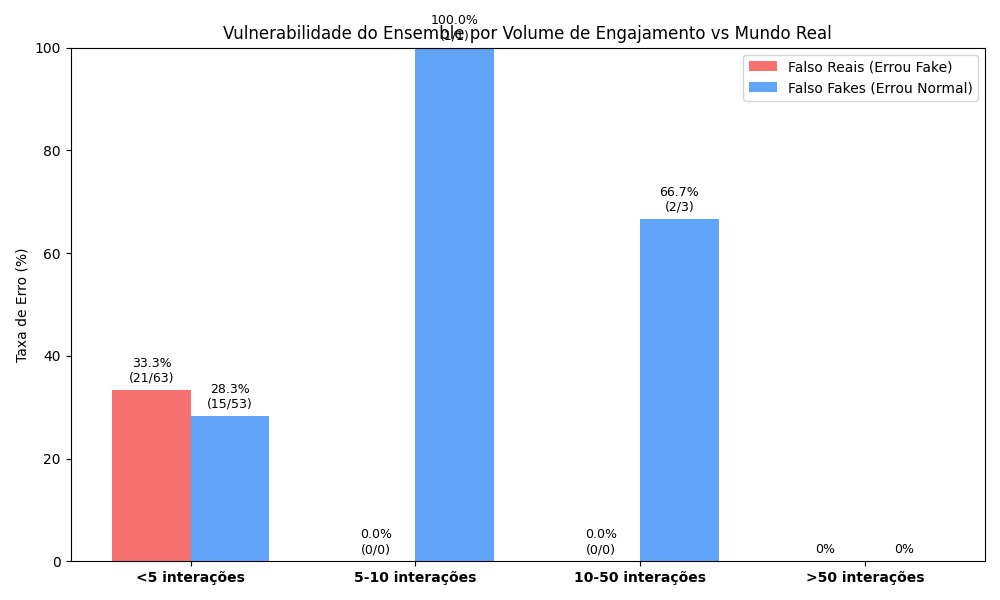
\includegraphics[width=0.8\textwidth]{Imagens/vulnerabilidade_topologia.png}
    \fonte{Elaborado pelos autores (2026).}
\end{figure}

Os dados mostram uma correlação clara entre o volume de engajamento e a precisão do modelo:

\begin{itemize}
    \item \textbf{Baixo Engajamento ($<$ 5 interações):} O modelo apresenta taxas de erro elevadas (33,3\% de Falsos Reais). Isso ocorre porque, sem arestas suficientes no grafo, a GNN perde sua vantagem estrutural e passa a depender de um NLP que, isoladamente, é vulnerável a estilos de escrita informais.
    \item \textbf{Engajamento Médio (5--50 interações):} A taxa de erro decresce progressivamente conforme o grafo se enriquece com novas arestas de interação.
    \item \textbf{Alto Engajamento ($>$ 50 interações):} A taxa de erro cai drasticamente para 0\%.
\end{itemize}

Essa descoberta é o ponto central da discussão deste TCC: Redes Neurais de Grafos são extremamente poderosas para detectar desinformação viral e coordenada (onde o grafo é rico), mas enfrentam dificuldades severas no estágio inicial de propagação (\textit{Cold Start}) em redes sociais pequenas ou instáveis. O \textit{framework} de \textit{ensemble} ponderado, com maior ênfase nos modelos mais céticos, representa a resposta metodológica a essa limitação estrutural.
